\documentclass[tikz,border=8pt]{standalone}
% Shared look for every TikZ diagram. Load with \input{../../tools/tikz-style.tex}
\usepackage[T1]{fontenc}
\usepackage{lmodern}
\renewcommand{\sfdefault}{lmr}  % diagrams use the same serif as the text
\usetikzlibrary{arrows.meta, positioning, shapes.geometric, calc, fit, backgrounds}
\definecolor{cblue}{HTML}{4C78A8}
\definecolor{corange}{HTML}{F58518}
\definecolor{cgreen}{HTML}{54A24B}
\definecolor{cred}{HTML}{E45756}
\definecolor{cpurple}{HTML}{B279A2}
\definecolor{cgrey}{HTML}{6B6B6B}
\tikzset{
  every picture/.style={font=\sffamily, line width=1.2pt},
  box/.style={draw=#1, fill=#1!12, rounded corners=4pt, align=center, inner sep=7pt, minimum height=1.1cm},
  box/.default=cgrey,
  arrow/.style={-{Stealth[length=3mm]}, draw=cgrey, line width=1.4pt},
  title/.style={font=\sffamily\bfseries\Large},
  note/.style={font=\sffamily\small, text=cgrey, align=center},
}
\AtBeginDocument{\hyphenpenalty=10000 \exhyphenpenalty=10000}

\begin{document}
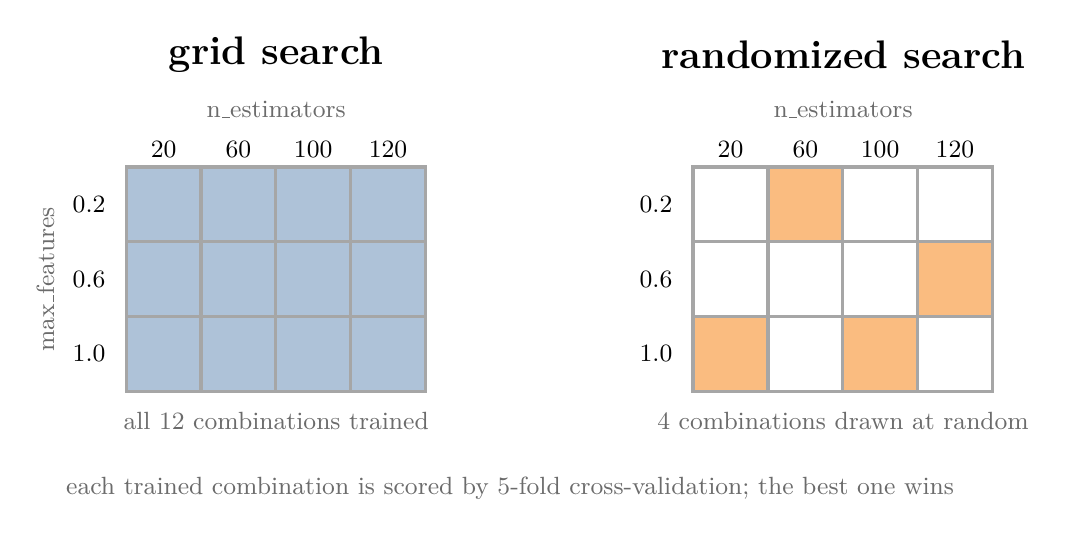
\begin{tikzpicture}[cell/.style={draw=cgrey!60, minimum size=0.95cm, inner sep=0pt},
  on/.style={cell, fill=cblue!45}, hit/.style={cell, fill=corange!55}]
  % \board{x}{title}{list of trained cells "col/row"}{style}
  \newcommand{\board}[5]{
    \begin{scope}[shift={(#1,0)}]
      \node[title] at (1.43,1.9) {#2};
      \foreach \c in {0,...,3} \foreach \r in {0,1,2} \node[cell] at (\c*0.95,-\r*0.95) {};
      \foreach \c/\r in {#3} \node[#4] at (\c*0.95,-\r*0.95) {};
      \foreach \v [count=\i from 0] in {20,60,100,120} \node[font=\sffamily\small] at (\i*0.95,0.7) {\v};
      \foreach \v [count=\i from 0] in {0.2,0.6,1.0} \node[font=\sffamily\small, anchor=east] at (-0.6,-\i*0.95) {\v};
      \node[note] at (1.43,-2.75) {#5};
    \end{scope}}
  \board{0}{grid search}{0/0,1/0,2/0,3/0,0/1,1/1,2/1,3/1,0/2,1/2,2/2,3/2}{on}{all 12 combinations trained}
  \board{7.2}{randomized search}{1/0,3/1,0/2,2/2}{hit}{4 combinations drawn at random}
  \node[note, rotate=90] at (-1.5,-0.95) {max\_features};
  \node[note] at (1.43,1.2) {n\_estimators};
  \node[note] at (8.63,1.2) {n\_estimators};
  \node[note] at (4.4,-3.6) {each trained combination is scored by 5-fold cross-validation; the best one wins};
\end{tikzpicture}
\end{document}
